\section{Mechanical design and locomotion system}
250 word + image

images/rover-front.png
images/rover-side.png
images/rover-top.png

\begin{figure}[htbp]
   \caption{\label{fig:rover} CAD view of the rover}
   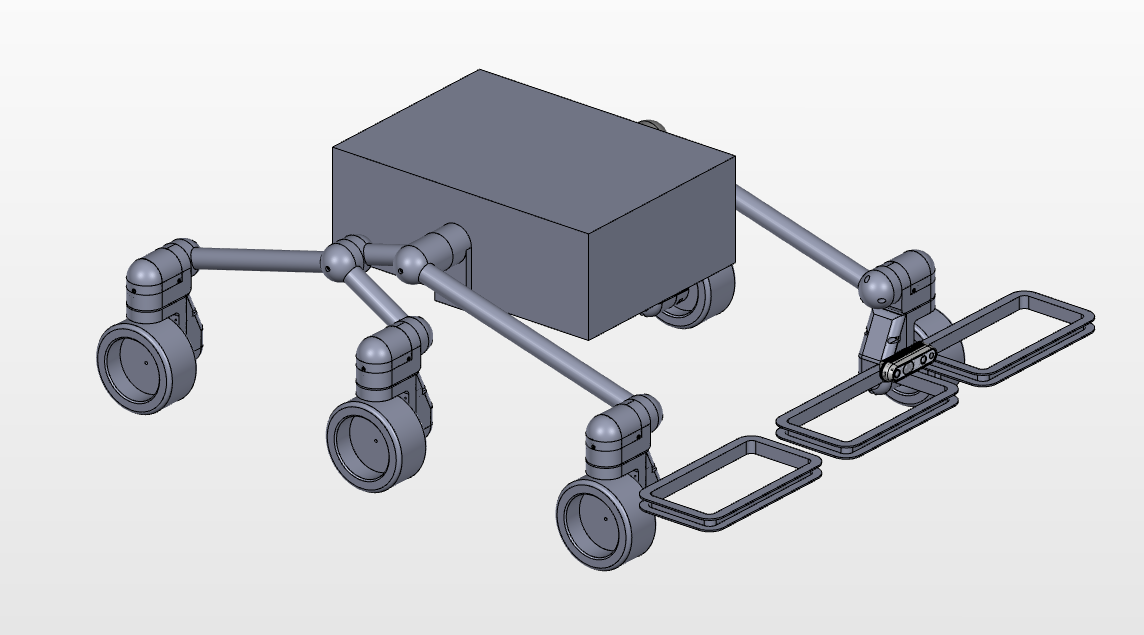
\includegraphics[width=\textwidth]{images/rover}
\end{figure}

\section{Sensors and landmine detection}
We detect landmines through two sensor measurements:
\begin{enumerate}
    \item a pulse induction metal detector to detect surface and buried landmines
    \item an RGBD sensor to detect surface landmines
\end{enumerate}

The metal detector is built around a resistor-inductor circuit formed by the coil.
We charge this coil with short pulses in the range of its characteristic time-constant $\tau = \frac{L}{R}$.
Then we measure the discharge signal and fit an exponential curve to it.
Three cases can arise:
\begin{enumerate}
    \item Nothing is observed, hence we only observe $\tau$ of the coil
    \item Non-ferromagnetic metal is near, hence we observe a shorter $\tau$ on the discharge curve because the eddy currents generated in the metal by electromagnetic stimulation decay the magnetic field faster
    \item Ferromagnetic metal is near, hence we observe a longer $\tau$ on the discharge curve because the ferromagnetic metal will be magnetized temporarily and retains the magnetic field longer
\end{enumerate}
In order to make this detection more reliable, we had to compensate for temperature drift on the measurement.
Driving the coil at high power heats it, which makes the resistance grow as $R = R_0 (1 + a T + a T^2)$.

A complementary detection mechanism is implemented using an RGBD sensor.
From the sensor data we build a local point cloud of the scene in front of the rover.
Then, we segment it to extract objects from the ground.
Objects that fit the geometric and color description of a landmine are logged.

\section{Electronic circuit and control system}
250 words + image

\section{Area navigation}
Our navigation is simple but open for extension.
The rover will be manually driven, however everything is such that the onboard computer could control the rover.
The idea is the cover the field in a grid pattern, while going around any landmines we encounter.

\section{Mapping}

To map the competition area, our robot will use a custom localization system that we developped.
Similarly to GPS, our system computes the rover's position by using the \gls{rtt} of a radio signal to several fixed beacons, of which the position is known.

We use Decawave's DWM1000 radio modem with a custom protocol to measure the distance.
This gives us a good distance measurement accuracy: $1 \sigma = \SI{3}{\centi\meter}$.

Since we know the distance to each fixed beacons, as well as their positions, we can compute the position of the robot.
This is done using an \gls{ekf}, using the distance to a point as a correction function.
For the prediction step, we originally planned to use an inexpensive \gls{imu}, similar to the ones found in mobile phones.
However we probably won't implement it, due to time constraints.

The system was already tested on a \SI{20}{\meter} by \SI{20}{\meter} open field at our workshop.
We got very good positioning results and reliability, although we lacked time to do a quantitative analysis of the measurement accuracy and precision.
According to simulation, we should be within \SI{10}{\centi\meter} of ground truth.
As the reliability so far is good, we will be using this system only for Minesweepers 2018.


\section{Rough environment handling}

250 words

\textbf{YOUTUBE VIDEO}
